%!TEX program = lualatex
\documentclass[11pt,a4paper]{article}
%\usepackage[utf8]{inputenc} % Allows Unicode characters
\usepackage[ngerman]{babel} % Handles German hyphenation and captions correctly
\usepackage{geometry}
\usepackage{array}
\usepackage{fontspec}
\usepackage{tgheros}
\setsansfont{texgyreheros}
\usepackage{hyperref}
\usepackage{setspace}
\usepackage{enumitem}
\usepackage{pgf}
\usepackage{url}
\usepackage{tikz}
\usepackage{amsmath}
\usepackage{pgfplots}
\pgfplotsset{compat=newest} % Nutzt die neuesten Features von pgfplots
\usetikzlibrary{plotmarks}
\usepackage{float}

\usepackage{graphicx}%images
\usepackage{subcaption} % Required for side-by-side subfigures

\usepackage{listings}
\usepackage{xcolor} % Für die farbige Gestaltung des Codes

\usepackage[protrusion=true,expansion=true]{microtype} % Verbessert die Typografie
%\usepackage[utf8]{inputenc}
\usepackage{amsfonts}
\usepackage{booktabs}

\overfullrule=5pt
% Hier definierst du das Design für den Code:
\lstset{
    backgroundcolor=\color{gray!5}, % Leichter grauer Hintergrund
    basicstyle=\small\ttfamily,     % Kleine, feste Schriftart
    breaklines=true,                % Automatische Zeilenumbrüche
    keywordstyle=\color{blue},      % MATLAB-Keywords werden blau
    commentstyle=\color{green!50!darkgray}, % Kommentare werden grün
    stringstyle=\color{purple},     % Strings werden lila
    numbers=left,                   % Zeilennummern links
    numberstyle=\tiny\color{gray},  % Kleine graue Zeilennummern
    stepnumber=1,                   % Jede Zeile nummerieren
    frame=single,                   % Ein einfacher Rahmen um den Code
    tabsize=4,                      % Tabulator-Breite
    showstringspaces=false          % Keine störenden Symbole in Leerzeichen
}

\geometry{
    a4paper,
    left=25mm,
    right=25mm,
    top=30mm,
    bottom=30mm
}

\definecolor{codegray}{rgb}{0.95,0.95,0.95}
\definecolor{commentgreen}{rgb}{0,0.6,0}

\lstset{
    backgroundcolor=\color{codegray},
    basicstyle=\ttfamily\small,
    breaklines=true,
    commentstyle=\color{commentgreen},
    keywordstyle=\color{blue},
    frame=single,
    rulecolor=\color{lightgray},
    language=bash,
    showstringspaces=false
}

\title{Laborprotokoll: Audiokodierung\\ \large Laboraufgaben LB-AK 01 bis LB-AK 04}
\author{Medientechnik Labor}
\date{\today}
\begin{document}

\maketitle
\tableofcontents
\newpage

\section{Einführung und Grundlagen}
Für die Bearbeitung der Laboraufgaben zur Audiokodierung werden die Programme \texttt{FFmpeg}, \texttt{ffprobe}, der \texttt{Nero AAC Codec} sowie \texttt{Audacity} verwendet. Sämtliche Kodierungsvorgänge werden über die Kommandozeile (CLI) durchgeführt und anschließend durch subjektive Hörtests sowie objektive Spektralanalysen bewertet.

\subsection{Praktische FFmpeg-Parameter}
Die folgenden Parameter sind für die Steuerung von Codecs und Containerformaten von zentraler Bedeutung:
\begin{table}[h!]
\centering
\begin{tabular}{ll}
\toprule
\textbf{Kommandozeilenparameter} & \textbf{Bedeutung} \\
\midrule
\texttt{-acodec <Format>} & Audio-Codec festlegen \\
\texttt{-vcodec <Format>} & Video-Codec festlegen \\
\texttt{-f <Format>} & Containerformat erzwingen \\
\bottomrule
\end{tabular}
\caption{Übersicht grundlegender Formatparameter in FFmpeg}
\end{table}

Abfrage unterstützter Formate und Codecs:
\begin{lstlisting}
# Liste der unterstuezten Containerformate abrufen
ffmpeg -formats

# Verfuegbare Audio- und Video-Codecs anzeigen
ffmpeg -codes
\end{lstlisting}

\subsection{Datenratensteuerung}
Die Regelung der Datenrate erfolgt mit dem Parameter \texttt{-b}, der vor dem jeweiligen Ausgabepfad definiert werden muss. 
\begin{table}[h!]
\centering
\begin{tabular}{ll}
\toprule
\textbf{Kommandozeilenparameter} & \textbf{Bedeutung} \\
\midrule
\texttt{-b:a <Datenrate>} & Datenrate des Audio-Codecs (z. B. 32k = 32 kbit/s) \\
\texttt{-b:v <Datenrate>} & Datenrate des Video-Codecs (z. B. 2000k = 2.000 kbit/s) \\
\bottomrule
\end{tabular}
\caption{Parameter zur Bitratensteuerung}
\end{table}

\subsection{Weitere nützliche CLI-Parameter}
\begin{table}[h!]
\centering
\begin{tabular}{ll}
\toprule
\textbf{Parameter} & \textbf{Bedeutung} \\
\midrule
\texttt{-an} & Audiospur wird entfernt (pro Ausgabe) \\
\texttt{-vn} & Videospur wird entfernt (pro Ausgabe) \\
\texttt{-y} & Existierende Ausgabedateien ohne Nachfrage überschreiben \\
\texttt{-re} & Eingabe-Streaming erfolgt möglichst in Echtzeit \\
\texttt{-stream\_loop -1} & Eingabedatei wird unendlich oft wiederholt (geloopt) \\
\bottomrule
\end{tabular}
\caption{Globale und spurrelevante Hilfsparameter}
\end{table}

\begin{figure}[H]
    \centering
    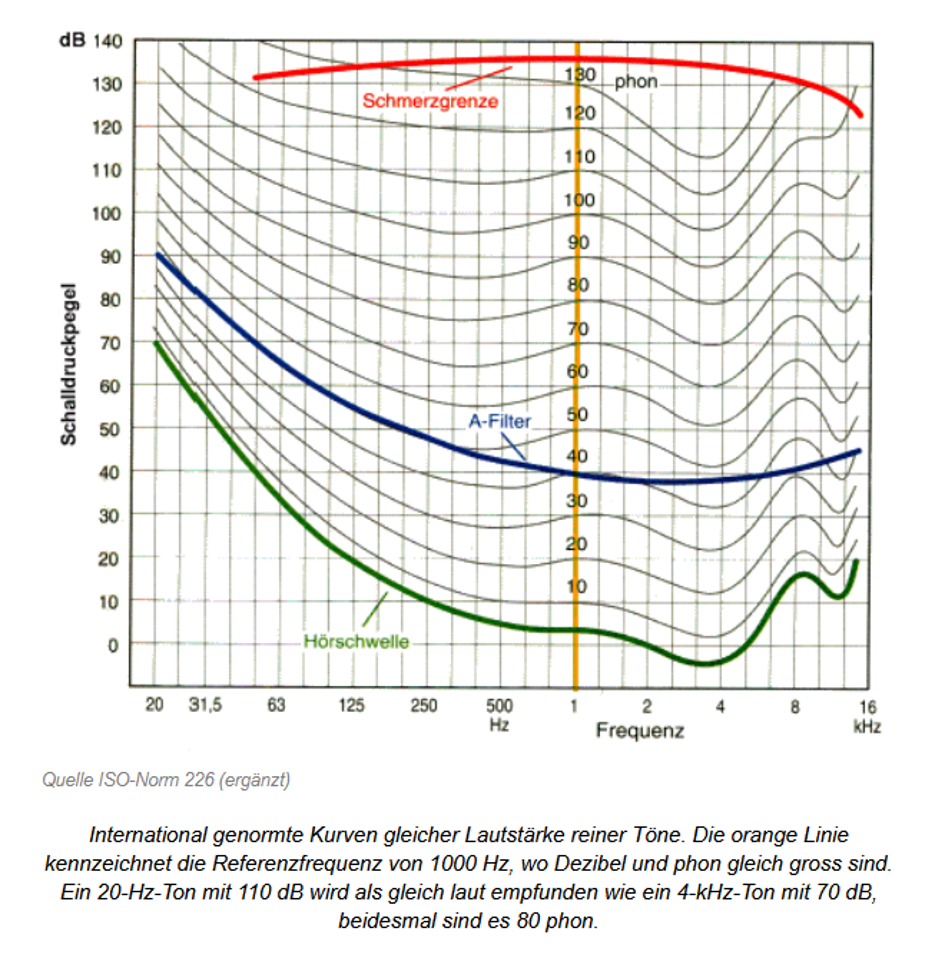
\includegraphics[width=0.7\textwidth]{Bilder/ISONORM226.png}
    \label{fig:img1}
\end{figure}
Warum wirkt manches leister? Vermutlich, weil die Hohen Frequenzen weggefiltert werden.
\newline
\newline
Schärfe und Rauheit:
\noindent „Wie scharf ein Audiosignal wahrgenommen wird, hängt hauptsächlich von der Umhüllenden des Spektrums und bei schmalbandigen Signalen von deren Mittenfrequenz
ab. Steigt die Anzahl an hohen Frequenzen im Signal bzw. steigt die Mittenfrequenz eines schmalbandigen Signals, so wirkt es schärfer.“
\newline
\newline
Tonhöhe:
\noindent „Die Tonhöhe kann mit der Grundfrequenz eines Klangs gleichgesetzt werden.“ \url{https://curdt.home.hdm-stuttgart.de/PDF/Brauner.pdf}



\newpage
\section{LB-AK 01: Standard-AAC-Kodierung mit FFmpeg}

\subsection{a) Kodierung in verschiedene Bitraten}
Die bereitgestellten WAV-Dateien (\texttt{music\_orig.wav} und \texttt{speech\_orig.wav}) werden mittels des standardmäßigen FFmpeg-AAC-Encoders in unterschiedliche Bitraten (16k, 32k, 64k) überführt.

Beispielhafte manuelle Befehle:
\begin{lstlisting}
ffmpeg -i beispiel.wav -c:a aac -b:a 16k beispiel_16k.aac
ffmpeg -i beispiel.wav -c:a aac -b:a 32k beispiel_32k.aac
ffmpeg -i beispiel.wav -c:a aac -b:a 64k beispiel_64k.aac
\end{lstlisting}

Zur Automatisierung kann folgendes Bash-Skript verwendet werden:
\begin{lstlisting}[language=bash]
#!/bin/bash
echo "Create Audio Files AAC from $1.wav"
for i in 16 32 64; do
     ffmpeg -i "$1.wav" -b:a ${i}k -acodec aac "${1}_output_${i}.aac"
     echo "Created ${i}k bitrate"
done
\end{lstlisting}

\subsection{Subjektive Qualitätsbewertung (Hörtests)}
Nach der Kodierung werden die Dateien mit einem Audioplayer mit dem Original verglichen. Dabei wird insbesondere auf Verständlichkeit, Rauschen, Verzerrungen, Hochtonverluste und Artefakte geachtet:

\begin{itemize}
    \item \textbf{Musiksignal (Music):}
    \begin{itemize}
        \item \textbf{16k:} Stark verzerrtes Signal, deutliches Knistern, kein klarer Ton vorhanden,Unterwasser Effekt.
        \item \textbf{32k:} Spürbare Besserung, jedoch weiterhin präsentes Rauschen und verzerrte Stimmen. Weniger schmerzhaft als bei 16k.
        \item \textbf{64k:} Stimmen wirken fast fehlerfrei ("`smooth"'), Instrumente klingen sauber und zeigen kaum noch Artefakte oder Verzerrungen.
    \end{itemize}
    \item \textbf{Sprachsignal (Speech):}
    \begin{itemize}
        \item \textbf{16k:} Sprache verständlich, roboterhaft/abgehackt, langgezogene Töne die schrill klingen
        \item \textbf{32k:} gut verständlich, leichte Verzerrungen
        \item \textbf{64k:} original klingt etwas klarer aber Artefakte sind kaum noch vorhanden
    \end{itemize}
\end{itemize}

\begin{verbatim}
Musik benötigt aufgrund ihrer hohen Dynamik, der vielen gleichzeitig spielenden Instrumente
und des breiten Frequenzspektrums deutlich mehr Bitrate als reine Sprache, um klar und ohne
Kompressionsartefakte zu klingen.
\end{verbatim}

\subsection{b) Vergleich mit MP3 (MPEG-1 Layer III)}
Ergänzend wird eine Kodierung bei einer Bitrate von 32 kbit/s mit MP3 durchgeführt. Beim Vergleich zeigt sich ein systematischer Unterschied in der Effizienz und Qualität bei niedrigen Bitraten: AAC (Advanced Audio Coding) liefert bei identischer Bitrate (32 kbit/s) eine hörbar bessere Dynamik und geringere Artefaktbildung im Hochtonbereich als MP3 (CBR vs. MPEG Average Bitrate).

\subsection{Analyse mittels ffprobe}
Hier zu sehen unter anderem Codec, Abtastrate (z. B. 48.000 Hz), Anzahl der Kanäle (Stereo vs. Mono), Bitrate sowie die exakte Spurdauer evaluiert.

\begin{figure}[H]
    \centering
    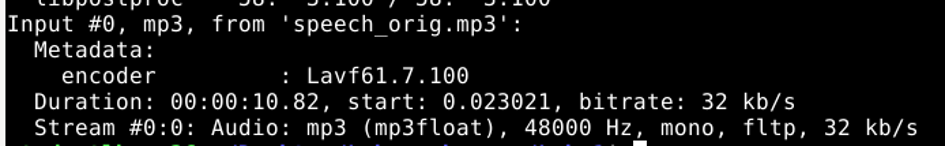
\includegraphics[width=0.7\textwidth]{Bilder/speechmp3.png}
    \label{fig:imgSpeechMP3}
\end{figure}
\begin{figure}[H]
    \centering
    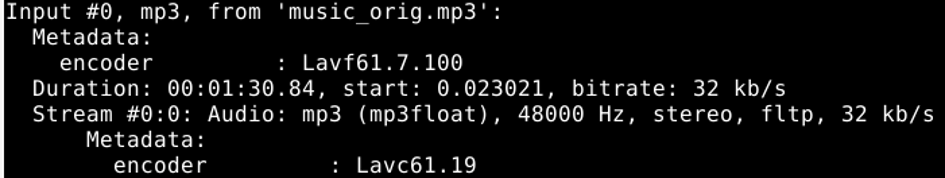
\includegraphics[width=0.7\textwidth]{Bilder/musicmp3.png}
    \label{fig:imgMusicMP3}
\end{figure}

\noindent Music:

\begin{figure}[H]
    \centering
    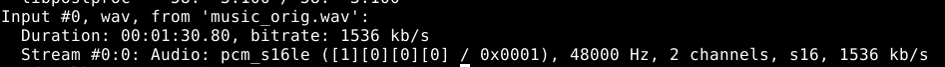
\includegraphics[width=0.7\textwidth]{Bilder/musicwav.png}
    \label{fig:imgMusicWAV}
\end{figure}
\begin{figure}[H]
    \centering
    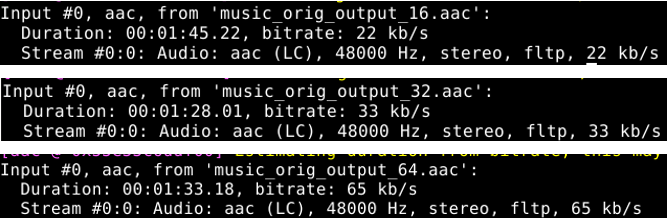
\includegraphics[width=0.7\textwidth]{Bilder/musicRates.png}
    \label{fig:imgMusicRates}
\end{figure}

\noindent Speech:

\begin{figure}[H]
    \centering
    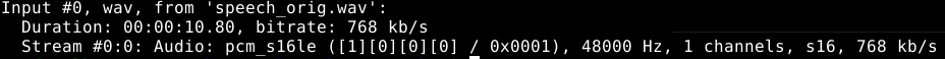
\includegraphics[width=0.7\textwidth]{Bilder/speechwav.png}
    \label{fig:imgSpeechWAV}
\end{figure}
\begin{figure}[H]
    \centering
    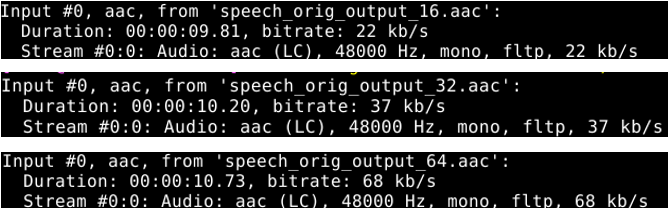
\includegraphics[width=0.7\textwidth]{Bilder/speechRates.png}
    \label{fig:imgSpeechRates}
\end{figure}

\begin{verbatim}
Unterschied Const and Variable Bit Rate
AAC Variable Bitrate
MPEG average bitrate

MP3 ist bei genau 32kb/s wohingegen AAC mehr nimmt. 
Wenig Unterschied, außer bei der Musik, an Stellen mit vielen verschiedenen Komponenten,
oder beim Gesang dort ist mehr knistern zu hören.
\end{verbatim}



\newpage
\section{LB-AK 02: Erweiterte AAC-Profile mit Nero AAC}
Unter Verwendung des externen Nero-Encoders werden fortgeschrittene Profile wie Low Complexity (AAC-LC), High-Efficiency AAC (HE-AAC v1) und HE-AAC v2 evaluiert.

\subsection{Befehlskonfigurationen}
\begin{itemize}
        \item \textbf{Für LC:}
    \begin{lstlisting}
neroAacEnc -if beispiel.wav -of beispiel_LC.mp4 -lc -br 32000
    \end{lstlisting}
    \item \textbf{Für HE-AAC (v1):}
    \begin{lstlisting}
neroAacEnc -if beispiel.wav -of beispiel_HE.mp4 -he -br 32000
    \end{lstlisting}
    \item \textbf{Für HE-AAC v2:}
    \begin{lstlisting}
neroAacEnc -if beispiel.wav -of beispiel_HEv2.mp4 -hev2 -br 32000
    \end{lstlisting}
\end{itemize}

Automatisierte Skriptverarbeitung über ein Hilfsskript (\texttt{./encode\_nero.sh}):
\begin{lstlisting}
./encode_nero.sh ../../music_orig.wav he
# Generiert automatisch: music_orig_he_16k.mp4, music_orig_he_32k.mp4, music_orig_he_64k.mp4, je nach Profil
\end{lstlisting}

\subsection{a) Vergleich von LC mit AAC bei gleicher Bitrate}
Sidenote: HE-AAC kombiniert AAC-LC mit \textit{Spectral Band Replication} (SBR), um bei extrem niedrigen Bitraten (z. B. 32 kbit/s) die höheren Frequenzbänder künstlich und datensparend zu rekonstruieren. HE-AAC v2 ergänzt dies um \textit{Parametric Stereo} (PS). Im subjektiven Vergleich schneiden HE-Profile bei geringen Bitraten deutlich vorteilhafter ab als Standard-AAC-LC.

\begin{itemize}
        \item \textbf{Für 16k: AAC knistert mehr, Unterwassereffekt, sehr intensiv (lauter)}
        \item \textbf{Für 32k: Nero feiner Unterschiede sind herauszuhören und es klingt lauter (aber nicht übertönend wie AAC 16k), Trommel-part mehr knistern als AAC, Gesang weniger knistern und roboterhaft}
        \item \textbf{Für 64k: Nero etwas klarer Ton, AAC beim Gesang schrillere Töne}
\end{itemize}

\subsection{b) Verbesserung von HE und HE v2 gegenüber LC}

HE: klarer, Töne besser differenzierbar, weniger knistern
HEv2: Gesang stimme wesentlich klarer und Hintergrund Geräusch währenddessen angenehmer.


\section{LB-AK 03: Objektive Frequenz- und Spektralanalyse}
Zur optischen Verifizierung der Kompressionsverluste wird in \textbf{Audacity} das Spektrum analysiert (\texttt{Analyse} $\rightarrow$ \texttt{Spektrum plotten...}).

\subsection{a) Vergleich der Spektren der Music File bei unterschiedlichen Bitraten}

Original WAV-Datei:
\begin{figure}[H]
    \centering
    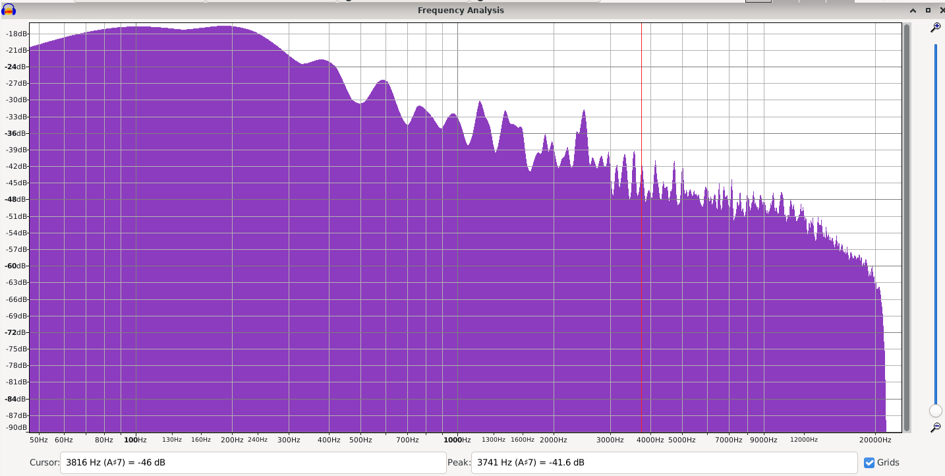
\includegraphics[width=0.9\textwidth]{Bilder/musicWavSpec.png}
    \label{fig:imgMusicWavSpec}
\end{figure}
\noindent Breites Spektrum von 0 bis 200kHz. Niedrige Frequenzen bis 400 Herz kaum gefiltert und flache Verläufe bis 1kHz
\newline

16kbit/s:
\begin{figure}[H]
    \centering
    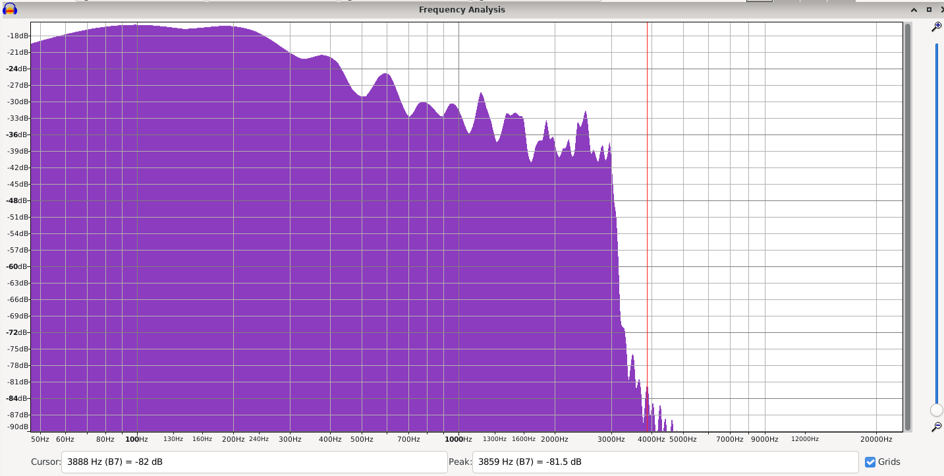
\includegraphics{Bilder/music16Spec.png}
    \label{fig:imgMusic16Spec}
\end{figure}
\noindent Ab 30kHz starker Abfall, Niedrige Frequenzen bis 300Hz wenig gefiltert, flache Verläufe bis 800Hz.
\newline

32kbit/s:
\begin{figure}[H]
    \centering
    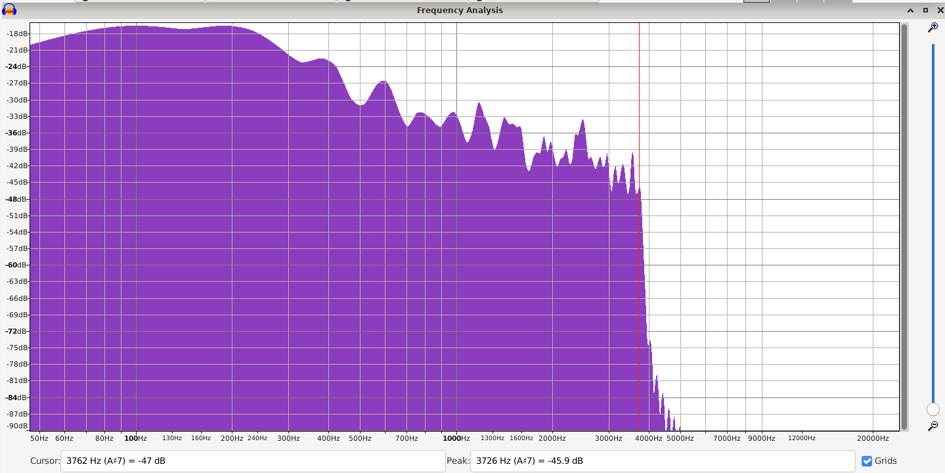
\includegraphics{Bilder/music32Spec.png}
    \label{fig:imgMusic32Spec}
\end{figure}
\noindent Starker Abfall bei 37kHz, flacher/welliger Verlauf bis 900Hz
\newline

64kbit/s:
\begin{figure}[H]
    \centering
    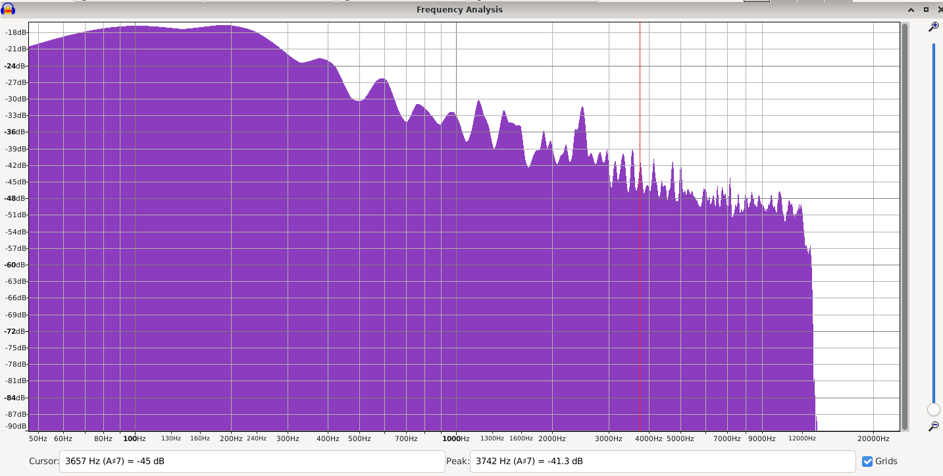
\includegraphics{Bilder/music64Spec.png}
    \label{fig:imgMusic64Spec}
\end{figure}
\noindent Bis 120kHz, flacher Verlauf bis 1kHz
\newline

Instrumente und Gesang verlieren durch das Abschneiden hoher Frequenzen ihre Klarheit, ihnen Fehlen die hohen Frequenzen. Es entstehen Artefakte.
Desto weniger gefiltert, desto fehlerfreier und glatter. Weniger Artefakte. Deckt sich im Wesentlichen mit der Subjektiven Wahrnehmung.

\subsection{b)Vergleich der Spektren bei unterschiedlichen Encodern (AAC-LC, HE-AAC, HE-AAC v2) bei gleicher Bitrate (32k)}
\indent AAC bei 32kHz:
\begin{figure}[H]
    \centering
    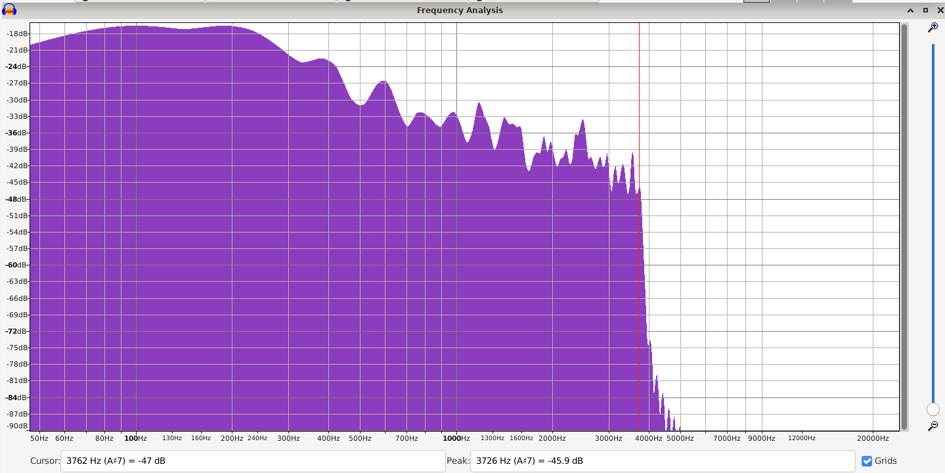
\includegraphics{Bilder/music32Spec.png}
    \label{fig:imgMusic32SpecVergleich}
\end{figure}
\noindent Starker Abfall bei 37kHz, flacher/welliger Verlauf bis 900Hz
\newline
\indent HE:
\begin{figure}[H]
    \centering
    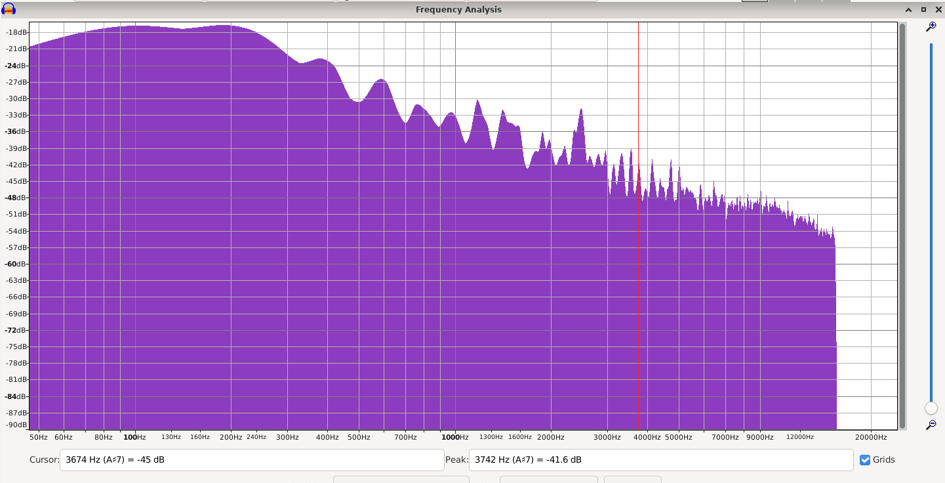
\includegraphics{Bilder/music32HE.png}
    \label{fig:imgMusic32SpecHE}
\end{figure}
\noindent Frequenzen bis 160kHz, selbe welligkeit.
\newline
\indent Hev2:
\begin{figure}[H]
    \centering
    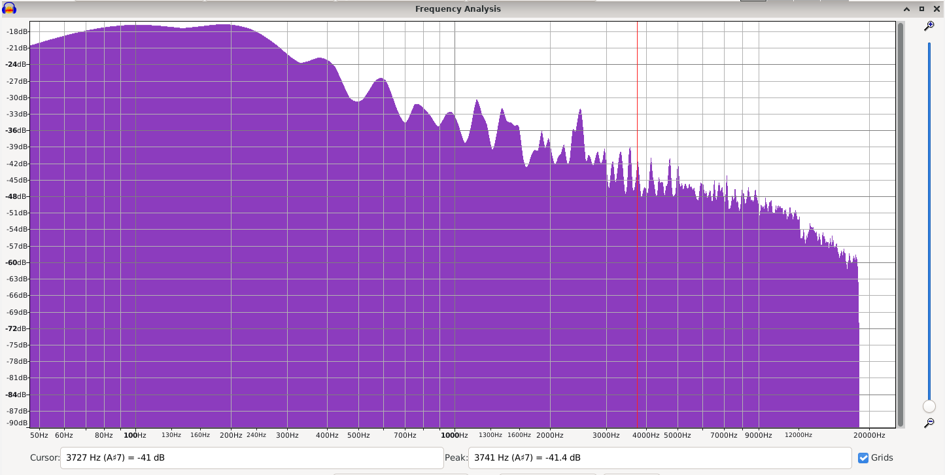
\includegraphics{Bilder/music32HE2.png}
    \label{fig:imgMusic32SpecHE2}
\end{figure}
\noindent Frequenzen bis 190kHz, selbe welligkeit.
\newline
\indent LC:
\begin{figure}[H]
    \centering
    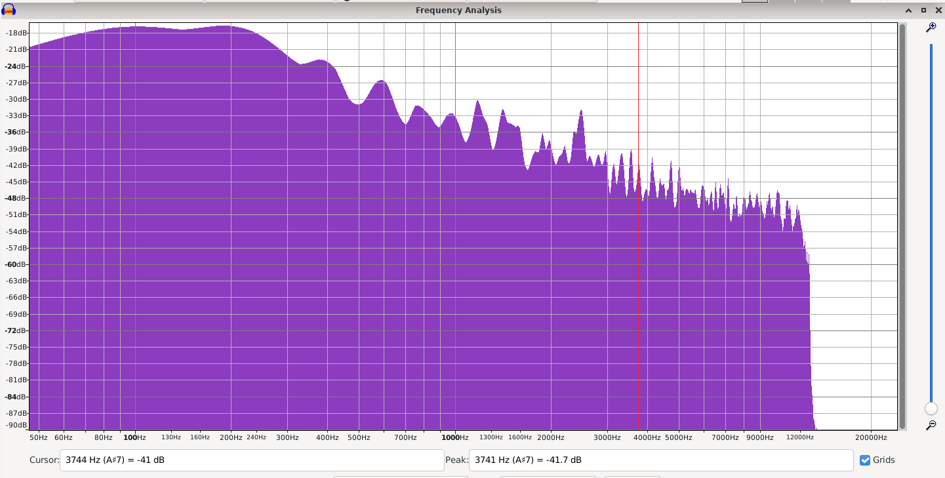
\includegraphics{Bilder/music32LC.png}
    \label{fig:imgMusic32SpecLC}
\end{figure}
\noindent Frequenzen bis 130kHz, selber Verlauf.
\newline

Größerer Unterschied zu LC, größere Filterung, hohe,spitze Ausschläge der hohen Frequenzen. Von HE auf HEv2 sind es vor allem hohe Frequenzen die genauer Abgetastet werden und das Frequenzspektrum ist auch breiter. Bei HE sind die Ausschläge schmaler und spitzer.
Dies führt dazu das HEv2 natürlicher, glatter und weniger kratzige Artefakte.


\subsection{Generelle Beobachtungen}
Bei sehr niedrigen Bitraten (16k/32k) schneiden Encoder alle Frequenzen oberhalb einer spezifischen Grenzschwelle ab, um Bits einzusparen. Bei 64k nähert sich der Frequenzverlauf deutlich dem Original an. Die HE-AAC-Dateien zeigen dank SBR auch bei 32k Signalanteile im oberen Spektralbereich, wohingegen Standard-LC-AAC oder MP3 dort steile Dämpfungsflanken aufweisen.

\newpage
\section{LB-AK 04}

\subsection{a)}
Installation der \texttt{libao} (Cross-Platform Audio Library)


\begin{itemize}
    \item \textbf{Kurzfassung:}
    \begin{itemize}
        \item \textbf{1.Archiv entpacken}
        \item \textbf{2.Konfiguration (./configure)}
        \item \textbf{3.Kompilieren (make)}
        \item \textbf{4.Installation (sudo make install)}
    \end{itemize}
\end{itemize}

\subsubsection{Schritt 1: Installation der System-Abhängigkeiten}
Da \texttt{libao} auf Linux-Systemen standardmäßig das ALSA-Subsystem (Advanced Linux Sound Architecture) zur Tonausgabe nutzt, müssen vor der Kompilation die entsprechenden Entwickler-Header-Pakete installiert werden:

\begin{lstlisting}[language=bash]
# Aktualisierung der Paketquellen und Installation der ALSA-Entwicklerbibliotheken
sudo apt update
sudo apt install -y libasound2-dev build-essential
\end{lstlisting}

\subsubsection{Schritt 2: Quellcode herunterladen, kompilieren und installieren}
Nachdem die Abhängigkeiten erfüllt sind, wird der Quellcode von \texttt{libao} (z.\,B. via Git oder als Tarball von Xiph.org) geladen, konfiguriert und systemweit installiert:

\begin{lstlisting}[language=bash]
# In das Verzeichnis des entpackten libao-Quellcodes wechseln
cd /pfad/zu/libao-source/

# Konfigurationsskript ausfuehren (ueberprueft Bibliotheken wie ALSA)
./configure --prefix=/usr/local

# Kompilation mit mehreren Kernen starten
make -j$(nproc)

# Systemweite Installation der Binaries und Header-Dateien
sudo make install

# Aktualisierung des Dynamic Linker Caches, damit die neue .so-Datei gefunden wird
sudo ldconfig
\end{lstlisting}

\subsubsection{Schritt 3: Kompilation und Ausführung des Programms}
Das fertige C-Programm muss gegen die mathematische Bibliothek (\texttt{-lm}) sowie die installierte \texttt{libao}-Bibliothek (\texttt{-lao}) gelinkt werden:

\begin{lstlisting}[language=bash]
# Kompilation des Beispielprogramms mittels GCC
gcc -o ao_example ao_example.c -lao -lm

# Ausfuehrung des Programms zur akustischen Verifikation
./ao_example
\end{lstlisting}
\subsection{b) Siehe Codefile}

\end{document}
